\documentclass[conference]{IEEEtran}
\usepackage{IEEEpreamble}

\usepackage{booktabs}
\usepackage{blindtext}
\usepackage{sepnum}
\usepackage{url}


\begin{document}
%
% paper title
% can use linebreaks \\ within to get better formatting as desired
\title{\textsc{Fuse}: A Reproducable, Internet-scale\\Dataset of Spreadsheets}

\author{
\IEEEauthorblockN{Titus Barik\IEEEauthorrefmark{1}\IEEEauthorrefmark{2}}
\IEEEauthorblockA{\IEEEauthorrefmark{1}ABB Corporation Research\\
Raleigh, North Carolina, USA\\
titus.barik@us.abb.com
}
\and
\IEEEauthorblockN{
Kevin Lubick,
Justin Smith,\\
John Slankas
Emerson Murphy-Hill}
\IEEEauthorblockA{
\IEEEauthorrefmark{2}North Carolina State University, Raleigh, USA\\
\{kjlubick, jssmit11, jbslanka\}@ncsu.edu,\\emerson@csc.ncsu.edu}
\and
\IEEEauthorblockN{Felienne Hermans}
\IEEEauthorblockA{Delft University of Technology\\
Delft, Netherlands\\
f.f.j.hermans@tudelft.n
}
}

\maketitle

\begin{abstract}
We submit a corpus consisting of 1.5 million spreadsheets, extracted using the Common Crawl corpus (based on Blekko). This corpus is compared against a proprietary index from a leading search engine company to measure representative against other commercial index. This corpus is intended to replace EUSES.
\end{abstract}
% IEEEtran.cls defaults to using nonbold math in the Abstract.
% This preserves the distinction between vectors and scalars. However,
% if the conference you are submitting to favors bold math in the abstract,
% then you can use LaTeX's standard command \boldmath at the very start
% of the abstract to achieve this. Many IEEE journals/conferences frown on
% math in the abstract anyway.

% no keywords




% For peer review papers, you can put extra information on the cover
% page as needed:
% \ifCLASSOPTIONpeerreview
% \begin{center} \bfseries EDICS Category: 3-BBND \end{center}
% \fi
%
% For peerreview papers, this IEEEtran command inserts a page break and
% creates the second title. It will be ignored for other modes.
\IEEEpeerreviewmaketitle

\section{Call for Papers}

Oops: we forgot to handle application/vnd.oasis.opendocument.spreadsheet.

\textbf{Data papers}. We want to encourage researchers to share their data. Data papers should describe data sets curated by their authors and made available to others. They are expected to be at most 4 pages long and should address the following: description of the data, including its source; methodology used to gather it; description of the schema used to store it, and any limitations and/or challenges of this data set. The data should be made available at the time of submission of the paper for review, but will be considered confidential until publication of the paper. Further details about data papers are available on the conference website. 

\begin{enumerate}
\item Description of the data.
\item Methodology used to gather it
\item Description of the schema used to store it
\item Limitations and Challenges of data set
\end{enumerate}

\section{Introduction}

Why are spreadsheets software?

Existing corpora with some limitations:
-Snapshot
-Reproducable
-Focused on one company
-Small
-Dated
-No metadata
-No analysis tool

We provide a corpus creation technique that overcomes many of these limitations!

Why is our data better?
-reproducable
-larger
-better meta data
-scales up (we release our scanning software)
-expands and stays up to date


Our contributions are 
\begin{enumerate}
\item A corpus of ??? spreadsheets pulled from the pubic web
\item A pipeline of tools that allows other researchers to more easily perform spreadsheet extraction and analysis at scale
\item A detailed set of metadata for this corpus and two other corpora [foo], [bar]  which allow researchers to make queries without having to download or analyze the entire spreadsheet corpus.  
\end{enumerate}


\begin{figure}[!t]
\centering
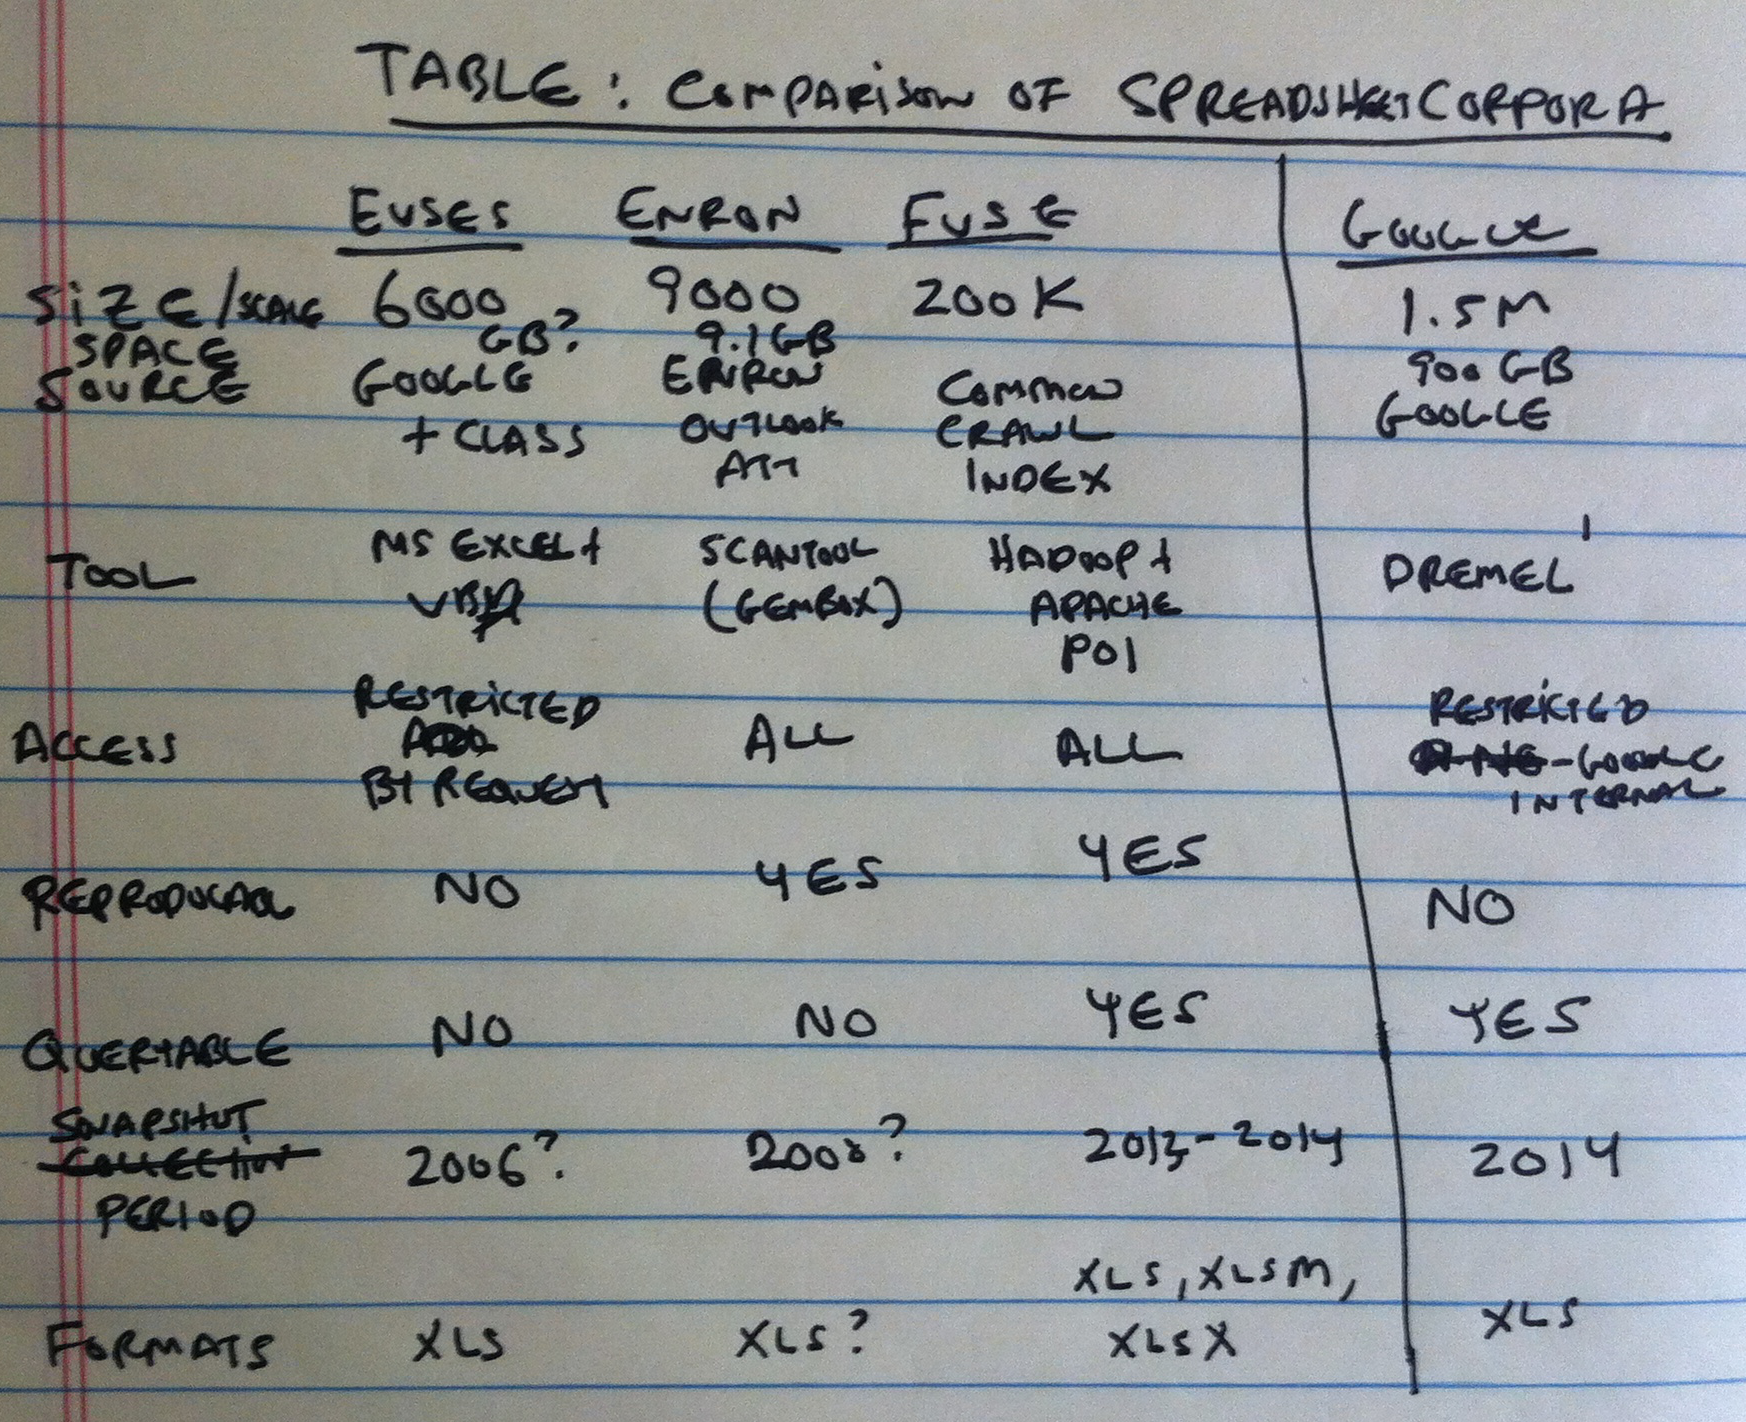
\includegraphics[width=0.5\columnwidth]{corpora}
\caption{Comparison matrix of available spreadsheet corpora. How does \textsc{Fuse} stack up?}
\label{fig:corpora}
\end{figure}

\begin{figure}[!t]
\centering
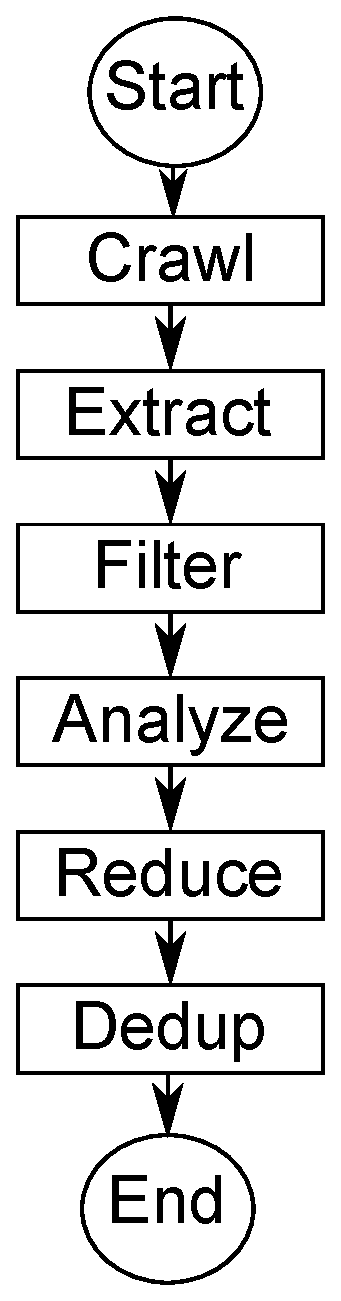
\includegraphics[width=0.4\columnwidth]{SpreadsheetPipeline}
\caption{MapReduce pipeline for spreadsheet extraction.}
\label{fig:mrpipeline}
\end{figure}

% TODO(tbarik)
%  This WAT file is okay, but the corresponding WARC record is corrupt:
% Put an example of this issue in the methodology.
%  {"WARC-Date":"2014-09-22T12:11:35Z","WARC-Record-ID":"<urn:uuid:0d670ac1-319f-42b0-89bf-7c52dd51e1dd>","Content-Length":1385,"WARC-Target-URI":"http://www.medcom.dk/dwn1514.xls","WARC-Content-Type":"application/json","Content":{"Envelope":{"Format":"WARC","WARC-Header-Length":"350","Block-Digest":"sha1:6JCTYB2KGCZ5YX63EFLECRMXB4KUBOQB","Actual-Content-Length":"263","WARC-Header-Metadata":{"WARC-Type":"request","WARC-Date":"2014-09-22T12:11:35Z","WARC-Warcinfo-ID":"<urn:uuid:1c4997f8-bc87-4ade-8efd-47f4cb8ce2a6>","Content-Length":"263","WARC-Record-ID":"<urn:uuid:81815bbd-d47d-4755-8e41-d820a1d05043>","WARC-Target-URI":"http://www.medcom.dk/dwn1514.xls","WARC-IP-Address":"91.193.139.41","Content-Type":"application/http; msgtype=request"},"Payload-Metadata":{"Trailing-Slop-Length":"4","HTTP-Request-Metadata":{"Headers":{"Accept-Language":"en-us,en-gb,en;q=0.7,*;q=0.3","Host":"www.medcom.dk","Accept-Encoding":"x-gzip, gzip, deflate","User-Agent":"CCBot/2.0 (http://commoncrawl.org/faq/)","Accept":"text/html,application/xhtml+xml,application/xml;q=0.9,*/*;q=0.8"},"Headers-Length":"261","Entity-Length":"0","Entity-Trailing-Slop-Bytes":"0","Request-Message":{"Method":"GET","Version":"HTTP/1.0","Path":"/dwn1514.xls"},"Entity-Digest":"sha1:3I42H3S6NNFQ2MSVX7XZKYAYSCX5QBYJ"},"Actual-Content-Type":"application/http; msgtype=request"}},"Container":{"Compressed":true,"Gzip-Metadata":{"Footer-Length":"8","Deflate-Length":"418","Header-Length":"10","Inflated-CRC":"505390695","Inflated-Length":"617"},"Offset":"654053188","Filename":"CC-MAIN-20140914011217-00240-ip-10-234-18-248.ec2.internal.warc.gz"}},"WARC-Refers-To":"<urn:uuid:81815bbd-d47d-4755-8e41-d820a1d05043>","Path":"common-crawl/crawl-data/CC-MAIN-2014-41/segments/1410657137046.16/wat/CC-MAIN-20140914011217-00240-ip-10-234-18-248.ec2.internal.warc.wat.gz"}

spreadsheets as end-user programmers; focus on how spreadsheets are useful for software engineerig


all the problems
euses sucks~~\cite{Fisher2005}

similar in size to other large corpora
representativeness against Google index
metadata

helps with tool evaluation

accessible -- getting this for yourself is a high cost maybe 5k

this set is reproducable
compared with existing data sets, it is new -- the others are more than a decade old.

even the enron corpus is 15000 spreadsheets -- whoopee. But it's good to compare against since it's a private corpus.

The contribution of this paper is:

\begin{itemize}
\item Foo
\end{itemize}

go to figshare
% http://figshare.com/articles/Enron_s_Spreadsheets_and_Related_Emails_A_Dataset_and_Analysis/1222882

\subsection{Subsection Heading Here}
Subsection text here.

need a fancy table

what metrics?

happy medium between euses and google

\subsubsection{Subsubsection Heading Here}
Subsubsection text here.

deliberate design decision to 
intentionally spluit the data into metadata and binary phases

\section{Data Extraction}
Initially, we extracted ??? candidate spreadsheets from the Common Crawl\footnote{\url{commoncrawl.org/}} index, which contains ???TB of uncompressed publicly available web crawl data. 
The Common Crawl data set is divided into several segments and is periodically supplemented with updated sections of the crawl. 
Our initial extraction targeted files that could potentially be spreadsheets, including files tagged with MSDN content types, and files with extensions containing ``.xls''.

Next we processed the files using Apache POI\footnote{\url{poi.apache.org/}} and Tika\footnote{\url{tika.apache.org/}} to identify the valid spreadsheets and extract metadata from each spreadsheet (see Section \ref{sec:schema}). After removing the invalid files detected in this step, ??? spreadsheets remained. Removing duplicates resulted in a final total of ??? spreadsheets. 


% https://publicsuffix.org/list/

% sebastien paper for other metrics a look inside common crawl
% http://blog.commoncrawl.org/2013/08/a-look-inside-common-crawls-210tb-2012-web-corpus/
% domain parsing is done using 

% https://publicsuffix.org/

limitation: truncation, 2 MB, 5 MB?

needed to create WAT index files

% dremel> select COUNT(doc.DocId) FROM docjoin.base WHERE doc.content.ContentType = 23;
% +------------------+
% | COUNT(doc.DocId) |
% +------------------+
% |          1635142 |
% +------------------+
% WARNING: Partition skipped
% WARNING: ~0.0% of data was not scanned (see "settings min_completion_ratio")
% 1 row in result set (319.28 sec)
% Scan rate: 37.38M rows/sec, SWE cost: 7.28138s

% dremel> select doc.DocId, RIGHT(doc.URL, 30), doc.Pagerank FROM docjoin.base WHERE doc.content.ContentType = 23 L
% IMIT 20;
% +----------------------+--------------------------------+--------------+
% | doc.DocId            | RIGHT(doc.URL, 30)             | doc.Pagerank |
% +----------------------+--------------------------------+--------------+
% | 18262361551973990081 | Noticias/210111pssufal2011.xls |        45696 |
% | 18262514318872388335 | E7%99%BB%E8%AE%B0%E8%A1%A8.xls |        53441 |
% | 18262628117481929248 | ameck-cd57ffgym.fr/file/31037/ |        49536 |
% | 18262462250520031836 | uation%20risque%20chimique.xls |            1 |
% | 18262515209375261799 | 9206/file/4%20LISTE%202014.xls |        51664 |
% | 18262601711327171729 | d_org=200054&id_dokumenty=1069 |        51318 |
% | 18262429851281169486 | loads/2009/11/distributori.xls |        47265 |
% | 18262677137761586621 | /03_Zahlungen_Schulversion.xls |        49376 |
% | 18262497829673811111 | FULL_SCHOOL_LIST_1982-1983.xls |        55771 |
% | 18098709049136093897 | 1_Guelleberechnungstabelle.XLS |        48219 |
% | 18098336056523698774 | 46658c58776252a270492189fd.xls |        51278 |
% | 18098420930462689378 | 2nd_and_3rd_Posting)_FINAL.xls |        46743 |
% | 18221693724751189184 | /stories/papka_bossa/rosta.xls |            1 |
% | 18221288433906859741 | mediaprodukciyu-22.12.2013.xls |        45065 |
% | 18221490419625251728 | 75817255013/files/sadowara.xls |        52813 |
% | 18221566511153360853 | ostnica-arhitektura_plosca.xls |        49301 |
% | 18221440248932413652 | 83%D1%81%D0%BA%D0%B8%D0%B9.xls |        44383 |
% | 18221602484570358598 | ents/0000000/44/25ichiran5.xls |        52927 |
% | 18221337705568163749 | es/201011/2010111710570042.xls |        52262 |
% | 18221462757268787142 | 20%D0%AF%D0%9D%D0%90%D0%9E.xls |        49763 |
% +----------------------+--------------------------------+--------------+
% 20 rows in result set (26.13 sec)
% Scan rate: 0.04M rows/sec, SWE cost: 6.4e-05s

For Summer 2013, Winter 2013, and March 2013, no pre-created WAT path files were available. To manually create this we did:



% aws s3 ls --recursive s3://aws-publicdatasets/common-crawl/crawl-data/CC-MAIN-2014-10/segments | awk '$4 ~ /wat/ {print $4}' > wat.summer2013.path

how did we decide to filter? MSDN content-type

% http://blogs.msdn.com/b/vsofficedeveloper/archive/2008/05/08/office-2007-open-xml-mime-types.aspx

google obtained from proprietary database query that extracted from google index all spreadsheets with content type application/ms-excel.

common crawl
segments -> subproblems

docjoiner

\emph{cleaning}

\section{Description of Spreadsheet Corpus}

% some ideas for things to show
% http://blog.commoncrawl.org/2012/05/


place a non-shitty graph here

% http://www.felienne.com/archives/3634
\begin{table}[!t]
%% increase table row spacing, adjust to taste
%\renewcommand{\arraystretch}{1.3}
% if using array.sty, it might be a good idea to tweak the value of
% \extrarowheight as needed to properly center the text within the cells
\caption{Comparison of \textsc{Fuse} and other spreadsheet corpora\label{tab:corpora}}
\centering
%% Some packages, such as MDW tools, offer better commands for making tables
%% than the plain LaTeX2e tabular which is used here.
\begin{tabular}{lllll}
\toprule
& \textbf{\textsc{Fuse}} & \textbf{EUSES} & \textbf{Enron} & \textbf{Google (est.)}\\
\midrule
Size ($n$) & a & 6,000 & 15,570 & $>$ 1.5 million \\
Space & b & c & 23.3\\
Research access & All & Restricted to researchers & All & Google internal\\
\bottomrule
\end{tabular}
\end{table}

A summary of your spreadsheet corpus can be found in Table~\ref{tab:corpora}.

\section{Results}

% stage 1 metadata

\section{Data Schema}
\label{sec:schema}
In this section, we describe the schema.
The metadata we collected for the indices was largely influenced by the summary statistics presented in \cite{Fisher2005}.  
For each spreadsheet, there are over 450 entries, so we will not list them all here.
In general, the entries summarize the contents of the cells.
To list a few examples, the number of times a given Excel function (such as SUM or VLOOKUP) is used, the total number of input or data cells, the number of numeric input cells, the number of formulas used more than 50 times, the most common formula used, etc.



how do you get it?

csv file
mongodb recordobject warc extracts


% TODO(tbarik): Switch this table.


\section{Dataset Limitations}

% https://gist.github.com/anonymous/8373f8a08a357146c20b

% https://groups.google.com/forum/#!topic/common-crawl/MV5yYWPWC_M
% As Kevin said, you might be able to get away using off the shelf search APIs, depending on exactly how much you want. One thing I will note though is that a MapReduce job over the relevant text data of Common Crawl won't cost hundreds of dollars, it would more likely cost somewhere between $30 and $60, possibly far cheaper if you run particularly optimized code.

% To combine all of them explicitly would just result in duplication of stored files, which is quite an issue when we're talking hundreds of terabytes.

% As all the files are stored in ARC or WARC, both web archive formats, the easiest way to combine them for your "full crawl" is to simply enumerate over all the files in all the crawls. This also allows you to decide what behaviour you would like (i.e. keep all pages, keep only the most recent pages, etc).

% https://groups.google.com/forum/#!topic/common-crawl/wb3jXh8x8Tg
% There are far more than 4.05 billion new web pages in the last three months. These crawls shouldn't be considered representative of how much of the web has changed or been updated in a given period of time as we only crawl a relatively small portion of the web. It also strongly depends on your definition of new, though that's a large and complicated situation all to itself.

relevance is dependent on common crawl definition of relevant

\section{Conclusion}
The conclusion goes here.

\section{Related Work}


\subsection{Why use spreadsheets}

\cite{Chambers2010} Use spreadsheet corpus + interviews to determine which features end-users use.

~\cite{Pinzger2012} Detecting code smells in spreadsheets. Analyze EUSES to study occurrence of smells.

~\cite{Badame2012} Refactor spreadsheet formula. Perform case study using EUSES dataset.

~\cite{Abraham2007} Support debugging spreadsheets

\subsection{What other corpora?}
EUSES~\cite{Fisher2005}

~\cite{Chen2013} Automatically extract relational data from spreadsheets. Extracted 410,554 spreadsheets from clue09 web crawl.

ENRON find citation <-- icse seip 2015



~\cite{Chen2013} Automatically extract relational data from spreadsheets. Extracted 410,554 spreadsheets from clue09 web crawl.


\textbf{Existing corpora.}
\textbf{Spreadsheet tools.}



% conference papers do not normally have an appendix


% use section* for acknowledgement
\section*{Acknowledgment}

This material is based upon work supported in whole or in part with funding from the Laboratory for Analytic Sciences (LAS). Any opinions, findings, conclusions, or recommendations expressed in this material are those of the author(s) and do not necessarily reflect the views of the LAS and/or any agency or entity of the United States Government.

% trigger a \newpage just before the given reference
% number - used to balance the columns on the last page
% adjust value as needed - may need to be readjusted if
% the document is modified later
%\IEEEtriggeratref{8}
% The "triggered" command can be changed if desired:
%\IEEEtriggercmd{\enlargethispage{-5in}}

% references section

\raggedright
% can use a bibliography generated by BibTeX as a .bbl file
% BibTeX documentation can be easily obtained at:
% http://www.ctan.org/tex-archive/biblio/bibtex/contrib/doc/
% The IEEEtran BibTeX style support page is at:
% http://www.michaelshell.org/tex/ieeetran/bibtex/
\bibliographystyle{IEEEtran}
% argument is your BibTeX string definitions and bibliography database(s)
\bibliography{library}


% that's all folks
\end{document}


